% Chapter Template

\chapter{Correct by Construction (CbyC) } % Main chapter title

\label{Chapter_CbyC} % Change X to a consecutive number; for referencing this chapter elsewhere, use \ref{ChapterX}

%----------------------------------------------------------------------------------------
\section{Overview}

The CbyC software development methodology proposes to limit software 
defects by \parencite{CbyCMan}:  
\begin{enumerate}
	\item making it difficult to introduce errors, and
	\item detecting and removing errors as early as possible.
\end{enumerate}

CbyC technique emphasises the use of mathematically rigorous tools. CbyC proposes
using mathematically formal language to define the specification and high-level design
of a system. This provides a precise description of the system's behaviour and a
precise model of its characteristics. Using a mathematical language also allows
the use of automated tools to verify the specification and design \parencite{CbyCMan}.

CbyC code is designed around information flow. The information flow is
defined using a contract-based notation. The contract-based notation is
used to define the abstract state of the program and the information relationships
across boundaries. CbyC proposes using programming languages and tools that allow
for the code and contracts to be validated using static analysis \parencite{CbyCMan}.
 
%----------------------------------------------------------------------------------------

\section{Correct by Construction Process}\label{CbyCDevWorkflow}

The CbyC process is described in terms of the artefacts it produces (Figure \ref{fig:CbyCDev}): 

\begin{itemize}
	\item System requirements specification;
	\item Formal specification;
	\item Formal design;
	\item System test specification;
	\item INFORMED design;
	\item Code;
\end{itemize}

Using the CbyC process every process artefact can be validated. The semantic gap 
between process artefacts are kept small. This makes it possible to show that later 
process artefacts conform to earlier process artefacts \parencite{Tokeneer}.

Here follows a description of each artefacts and how it is created.

\begin{figure}[H]
	\centering
	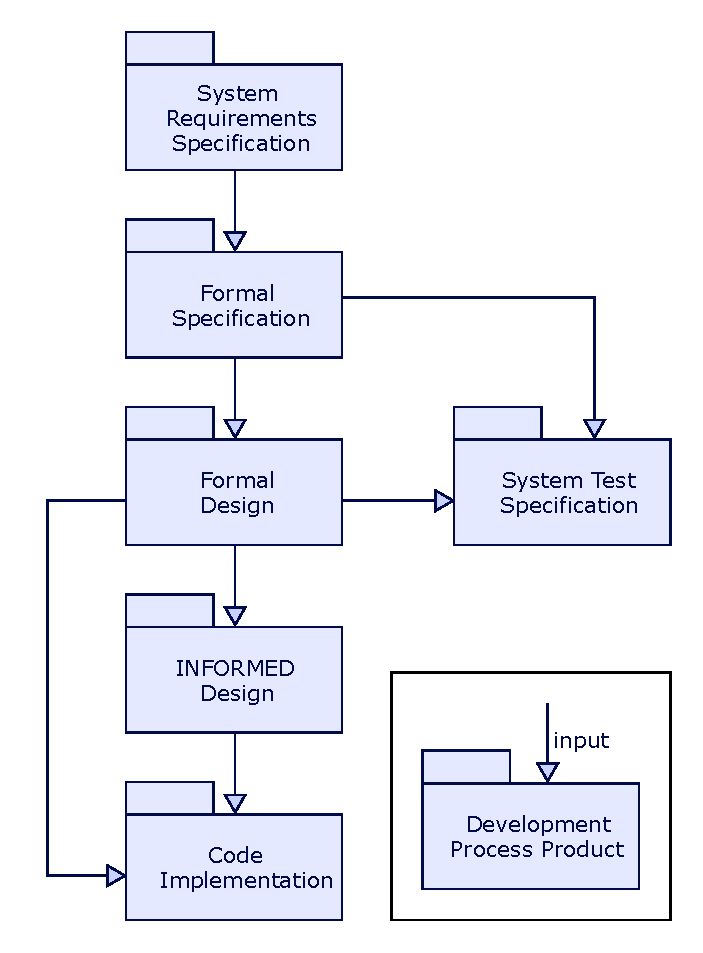
\includegraphics[scale=0.75]{Figures/CbyC_process.pdf}
	\decoRule
	\caption{CbyC process artefacts.}
	\label{fig:CbyCDev}
\end{figure}

\subsection{System Requirements Specification}

Requirements analysis identifies the needs of the stakeholders, the desired 
behaviour of the system, and any non-behavioural system characteristics \parencite{Tokeneer}. 

Requirements management extends throughout the system's development, but it is 
most significant at the beginning, where it is used to identify \parencite{Tokeneer}:
\begin{itemize}
	\item the stakeholders (who have an interest in the development and use of the system);
	\item the system boundary (to clarify the scope of the project and the interfaces to external systems);
	\item the expected use (in terms of interactions between users and the system);
	\item system properties (such as security properties, performance properties, etc).
\end{itemize}

Each requirement should be traceable through every process artefact \parencite{Tokeneer}.
The requirements are compiled into the System Requirements Specification document.

The System Requirements Specification is created to \parencite{Tokeneer}:
\begin{itemize}
	\item early in the project clarify the system's boundary (what is in scope 
		and what is out of scope, and the necessary interfaces to external systems);
	\item agree on the system requirements with all of the stakeholders;
	\item document the requirements with enough procession so that the Formal 
		Specification can be developed with minimal customer input;
	\item clarify and document the assumptions about the behaviour of the environment
		external to the system;
	\item identify and manage conflicting expectations between stakeholders.
\end{itemize}

\subsection{Formal Specification}

The Formal Specification unambiguously describes what the system
will do. This helps the developer and client gain a common understanding
of the system \parencite{Tokeneer}.

The level of abstraction is important. The Formal Specification should not describe 
the system's implementation. Internal details are deliberately left abstract. 
Interactions with the external environment are specified, but may also be abstract \parencite{Tokeneer}.

The Formal Specification is written in mathematical notation with an English 
narrative. The specification is divided into small components that can be reasoned
about individually. The small components are then combined to describe the system
as a whole \parencite{Tokeneer}.

The Formal Specification is created because it \parencite{Tokeneer}:
\begin{itemize}
	\item provides an unambiguous description of what the system does. This is
		important for client approval of the system's behaviour;
	\item can be shown to be complete;
	\item can be formally verified and proven consistent.
\end{itemize}

\subsection{Formal Design}

The Formal Design elaborates on the abstract aspects of the Formal 
Specification to explain how the system will be implemented. The Formal Design 
describes the system in terms of concrete state and operations using types that
are easily implementable. The Formal Design is the source of the required functional
behaviour used during implementation  \parencite{Tokeneer}.

The Formal Design is written in the same mathematical notation as the Formal Specification.
This means that the Formal Design can be formally verified and errors can be uncovered
before implementation starts \parencite{Tokeneer}.

The Formal Design is created because it \parencite{Tokeneer}:
\begin{itemize}
	\item provides an unambiguous description of how the system will accomplish what the Formal Specification requires;
	\item can be shown to be complete;
	\item can be formally verified and proven consistent.
\end{itemize}

\subsection{System Test Specification}

The systems tests described in the System Test Specification has to show that the system implements the 
behaviours described in the Formal Specification. System tests are more complete than 
acceptance tests. Acceptance tests only have to show that the system functions as described in the 
System Requirements Specification. System Testing aims to achieve 100\% coverage of the Formal 
Specification so that all behaviours described in the Formal Specification are executed at least once \parencite{Tokeneer}.

The Formal Design is a refinement of the Formal Specification. Therefore the Test
Specification can also be written against the Formal Design if you want to tests 
details of the design \parencite{Tokeneer}.

All system tests are specified in the System Test Specification before being executed.
The tests are specified as scenarios that can occur during typical system usage. 
The System Test Specification documents the expected outcome of the test. 
Each system test is linked to functionality described in the Formal Specification/Design\parencite{Tokeneer}.

Where code coverage metrics are needed, it can be done during the System testing. 
This allows us to question the use of any code that cannot be covered
by a system test \parencite{Tokeneer}.

System tests are specified because \parencite{Tokeneer}:
\begin{itemize}
	\item system tests focuses on testing the behaviour of the whole system against
		the expected (specified) behaviour;
	\item system tests find faults caused by interaction of the system's modules;
	\item system tests complement static analysis by confirming the system's dynamic behaviour.
\end{itemize}

\subsection{INFORMED Design}
CbyC design methodology is based on information flow. The information flow is 
defined using contract-based notation. The contract-based notation is used to
define the abstract state of the program and the information relationships across
boundaries \parencite{CbyCMan}.

The \textbf{IN}formation \textbf{F}low \textbf{OR}iented \textbf{ME}thod of
object \textbf{D}esign (INFORMED) design provided an architectural framework
in which to perform the implementation. Consideration of information flow at the
design stage results in programs with the desirable properties of abstraction, 
encapsulation, high cohesion and loose coupling \parencite{Tokeneer}.

The INFORMED design aids maintenance and upgrades of the software by providing a
route-map from the Formal Design to the code \parencite{Tokeneer}.

An INFORMED Design is created because it \parencite{Tokeneer}:
\begin{itemize}
	\item focuses on the system architecture and ensures that the architecture 
		fits the information flow model;
	\item provides the mapping from the Formal Design to the Code before writing
		the code.
	\item complements the Formal Design without duplicating functional information.
\end{itemize}

\subsection{Code}
We start by writing the module specification. The specification is the public 
interface and the contracts governing the global state of the module. The contacts
specify how inputs are allowed to influence outputs \parencite{Tokeneer}. 

After writing the specification we implement the module body. The Formal Design is
detailed enough to make the mapping from the design to the code simple 
\parencite{Tokeneer}.

Modules providing infrastructure are developed early. Modules are implemented 
in an order that allows system functionality to be added incrementally. This
means that a basic system can be built as soon as possible and functionality is 
added in subsequent builds. This has the advantage of addressing code integration
risks as early as possible \parencite{Tokeneer}.

By using languages that allows static analysis we can evaluate the code 
contracts at build time, if the code builds, it is correct as specified by the
contracts \parencite{Tokeneer}.